\documentclass[12pt]{article}
\pagestyle{plain}
\usepackage[pdftex]{graphicx}
\usepackage{fullpage,graphicx,psfrag,url,caption}
\usepackage{amsmath,amsfonts,amssymb}
\usepackage{enumerate}

\topmargin=-0.5in
\textheight=9in
\oddsidemargin 0in
\evensidemargin 0in
\textwidth 6.5in
\renewcommand{\topfraction}{0.9}
\renewcommand{\dbltopfraction}{0.9}
\renewcommand{\textfraction}{0.1}
\newcommand{\sint}{sin(\theta/2)}
\newcommand{\cost}{cos(\theta/2)}
\newcommand{\lb}{\left[}
\newcommand{\rb}{\right]}
\begin{document}

{\parindent 0pt
BIOE165, Fall 2013\\
 Medical Imaging Signals and Systems\hfill Yigong Zhang \vskip 0.8in}

\begin{center}
{\Large\em HW10 Solution }\\[0.7in]
\end{center}

% this is a comment

\section*{Problem 1}

\begin{enumerate}[a)]
\item PET resolution is limited by the following factors:
	\begin{itemize}
	\item The finite size of the detector
	\item Positrons travel before annihilation
	\item Annihilated photons are not strictly $180\,^{\circ}$ apart
	\end{itemize}
\item The most damaging factor is the finite size of the detector
\item 
\begin{align*}
g(\theta, l)_{blur} &= \delta [x \cos(\theta)+y \sin(\theta)- l] \ast \sqcap(\frac{l}{w})
\\g(\theta, l)_{blur} &=\sqcap[\frac{x \cos(\theta)+y \sin(\theta)- l}{w}]
\end{align*}

\item The detector width is proportional to the diameter of the ring if the detector number keeps constant. And the resolution is proportional to the detector width. Thus, if the diameter of the ring is scaled down by a factor of 4, the resolution will be improved by a factor of 4.
				
\end{enumerate}

\section*{Problem 2}
There are a lot more attenuation happening in SPECT than in PET because of SPECT's low energy gamma-rays. So in SPECT, we have a lot to correct. But in PET, all we care is 511 keV photons. We can reject the background by putting an energy windows.

\section*{Problem 3}
Since the resolution is mainly contributed by the width of the detector. The 2D impulse response can be approximated as:
\begin{align*}
h(x,y) &= circ(r)|_{r =\sqrt{x^2+y^2}}
\end{align*}

\section*{Problem 4}
\begin{enumerate}[a)]
\item The nuclear magnetization in water is:
\begin{align*}
M_0 &= \frac{N \gamma^2 \bar{h} I_z(I_z + 1) B_0}{3kT}
\end{align*}
we know that $\frac{N \gamma^2 \bar{h} I_z(I_z + 1) }{3kT} = 3.25 \times 10^{-3} \, A/m$ for protons in water at $37\,^{\circ}$
\begin{align*}
M_0 &= 4.875 \times 10^{-3} A/m
\end{align*}

\item 
\begin{align*}
\emph{M} &= \chi \emph{H}
\\\emph{M} &= \chi \frac{B}{\mu_0}
\\\emph{M} &= 1\times10^{-5} \, \frac{1.5}{4\pi \times 10^{-7}} \,A/m
\\\emph{M} &= 12 \,A/m
\end{align*}

\item Since there's no precession for molecular diamagnetic magnetization, we are not gonna be able to extract information of the object in frequency, like what we do in MRI.

\end{enumerate}
		
\section*{Problem 5}
\begin{align*}
\omega &= \bar{\gamma} \cdot B
\\\omega &= \bar{\gamma} \cdot (B_0 + G \cdot x) 
\end{align*}
%\\\Delta \omega &= \Delta \bar{\gamma} \cdot B_0
\begin{center}
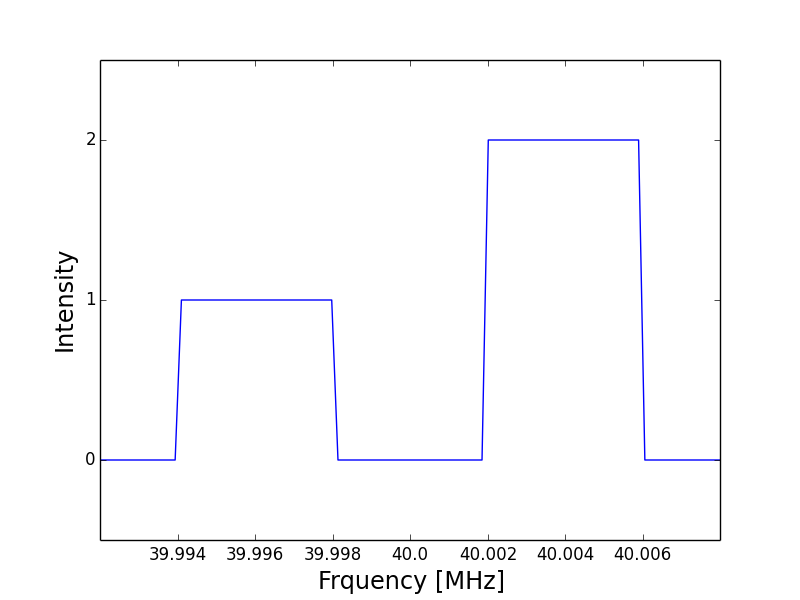
\includegraphics[width=0.8 \textwidth]{p5.png}
\end{center}
\captionof{figure}{Spectrum of NMR signal}


\section*{Problem 6}
\begin{enumerate}[a)]
\item The two radio emitters have different frequency. So we can choose the channel by demodulating the signal at different frequency.

\item How we distinguish the radio emitters is exactly how we use MRI to image the nucleus density in our body. We are trying to resolve them in frequency rather than time. 
\end{enumerate}

\end{document}

